\documentclass[zad,zawodnik,utf8]{sinol}
\usepackage{tikz}

\title{Nieskończone drzewko}
\id{nie}
\author{JT} % Autor zadania
\pagestyle{fancy}
\iomode{stdin}
\etap{początkująca}
\konkurs{XI obóz informatyczny}
\day{?}
\date{??.09.2015}
\RAM{32}
 
\begin{document}
\begin{tasktext}%
    Mamy pełne, nieskończone drzewko binarne. Należy obliczyć długość ścieżki z wierzchołka $a$ do $b$. 
    Zakładamy, że długość każdej krawędzi wynosi 1, a wierzchołki ponumerowane są kolejnymi liczbami $1, 2, \ldots$ 
    poczynając od korzenia.

\begin{figure}[h!]\centering
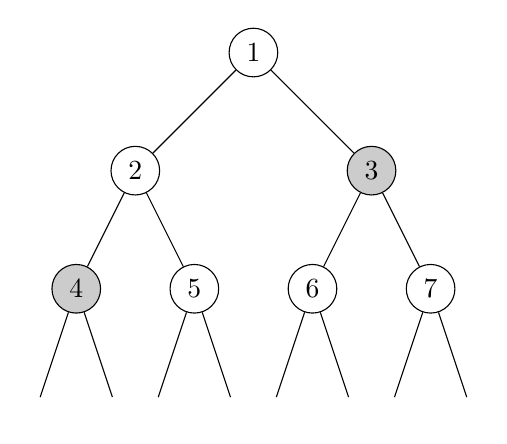
\begin{tikzpicture}[
  level distance=1.5cm,
  level 1/.style={sibling distance=3cm},
  level 2/.style={sibling distance=1.5cm},
  level 3/.style={sibling distance=1cm},
  level 4/.style={sibling distance=1cm}]
  
  \node[style={draw,circle}] {$1$}
    child {node[style={draw,circle}] {$2$}
      child {node[fill=black!20, style={draw,circle}] {$4$}
        child {node {$ $}}
        child {node {$ $}}
      }
      child {node[style={draw,circle}] {$5$}
        child {node {$ $}}
        child {node {$ $}}
      }
    }
    child {node[fill=black!20, style={draw,circle}] {$3$}
      child {node[style={draw,circle}] {$6$}
        child {node {$ $}}
        child {node {$ $}}
      }
      child {node[style={draw,circle}] {$7$}
        child {node {$ $}}
        child {node {$ $}}
      }
    };
\end{tikzpicture}
\end{figure}
    \noindent
    Przykładowo, długość ścieżki, pomiędzy wierzchołkiem numer $3$ i $4$ wynosi trzy.

\section{Wejście}
    Pierwszy i jedynym wiersz wejścia zawiera dwie liczby całkowite $a, b$ ($0 < a, b < 2 \cdot 10^9$).

\section{Wyjście}
    Pierwszy i jedyny wiersz wyjścia powinien zawierać jedną liczbę całkowitą, 
    równą długości ścieżki z $a$ do $b$.
\makecompactexample


\end{tasktext}
\end{document}
